
\documentclass[bsc,frontabs,twoside,singlespacing,parskip,deptreport]{infthesis}
\usepackage{eurosym}
\usepackage{graphicx}
\usepackage{hyperref}
\hypersetup{unicode=true,
			colorlinks=true,
			linkcolor=black,
			urlcolor=cyan,
            pdfborder={0 0 0},
            breaklinks=true}
\urlstyle{same}

\begin{document}

\title{RegEx Search \& Replace Extension for Chrome and Firefox}

\author{Dalimil Hajek}

\course{Computer Science}
\project{BSc Hons Project Report}
\date{\today}

\abstract{
The aim of this project was to build a browser extension to allow users to search and replace text with regular expressions in editable text input fields of web pages.

After evaluating existing extensions that were unsuccessfully attempting to implement this functionality, the new extension has been carefully designed, developed, and finally successfully released for Chrome and Firefox browsers.

In addition to the future-rich search and replace function, this plugin also adds the ability to save favorite patterns, store search history, or predefine text templates that can be inserted into the editable area of a page.

The software followed an iterative development process, where user feedback was collected via several means, including Google Analytics, which was used to track user interaction, and a support website used to collect user feedback comments.

After the initial release, about twenty updates have been subsequently released over the span of a few months. This iteration was further supported by automated tests of several kinds.

The extension has received excellent reviews and at the time of writing has over 3000 weekly users (users from both browsers combined).
}

\maketitle

\section*{Acknowledgements}
Thanks to
\begin{itemize}
\item
  Boris Grot - for supervising the whole project, and making important feature suggestions leading up to the first official releases of the extension on the Chrome and Firefox web stores
\item
  Michael O'Boyle - for making suggestions, especially regarding Google Analytics
\item
  Christoph Metze - for finding several important bugs that subsequently led to releases \texttt{1.3.2}, \texttt{1.3.3}, and \texttt{1.3.4}
\item
  Daniel Tomberlin - for pointing out a use case when trying to search across multiple single-line inputs, and for updating his web store rating and review after I implemented it in \texttt{1.3.6}
\item
  GitHub user \href{https://github.com/MarkRH}{MarkRH} - for finding a bug that was later fixed in \texttt{1.1.3}
\item
  StackOverflow user \href{https://stackoverflow.com/users/3959875/woxxom}{wOxxOm} - for suggesting \texttt{Document.execCommand} API that I used to fix issues with templates in \texttt{1.2.0}
\end{itemize}

And also thanks to all those people who submitted user feedback or
reviews.

\standarddeclaration

\tableofcontents
\listoffigures

\chapter{Introduction}
Modern web browsers allow users to find text in a web page, but when it comes to editable text areas that are often used on blogging platforms, online forums, social media, and email web clients, as a form of user input, none of the existing browsers allow users to also replace the found occurrences.
 
The aim of this project was to build an extension that adds this browser functionality. The tool allows users to find and replace text in editable text input fields of web pages, and includes a large set of features and search options, including regular expression support and occurrence highlighting.

\section{Motivation}
Search and replace functionality can be extremely useful when composing long emails, writing posts on social media, online forums, or blogging platforms, as well as in any email web clients. 

The most frequent use cases are:
\begin{itemize}
\item Fixing a typographical error -- A word or a phrase may have been used several times with the wrong spelling. This can reoccur several times in a forum post or an email, and it would be convenient to replace everything at once.

This also includes fixing unreadable characters in blog entries such as {\it \^{A}\euro\r{?}}, due to a change in encoding or some unintended text handling.

\item Normalizing incorrectly formatted text -- Regular expressions can be used to detect formatting errors such as multiple spaces before a period, missing upper-case letter, various metric unit formatting errors, and similar. Search and replace extension supporting regular expressions can quickly find and fix these.

\item Renaming a phrase -- Often a word or a phrase that occurs several times throughout a text needs to be corrected or substituted (perhaps using a synonym or a wording that sounds better)
\end{itemize}

Without having a browser extension for search and replace, one could imagine a solution where all text is copied and pasted into an advanced text editor, fixed using the built-in search and replace function, and copied back into the web page input field.

In addition to being a lengthy and time consuming process, this method would in many cases lose all text formatting, because more advanced editable text elements on the web may contain images, emojis, and text containing many formatting tags, which would not be preserved during the copy-pasting.

Additional motivation behind the development of this project was to add search-and-replace related features that are missing even from the more advanced text editors. One of them is storing the search history, and also being able to save favorite search patterns, that can later be quickly accessed. Both of these would save time and increase user productivity.

\section{Existing Extensions}
Web browsers support standard search functionality for any text on a page but no browsers have the find \& replace functionality. Users have asked for this feature on Google Chrome forums\footnote{Google Chrome Forum link: \href{https://productforums.google.com/forum/\#!topic/chrome/Y4UORlpdYfo}{https://productforums.google.com/forum/\#!topic/chrome/Y4UORlpdYfo}}, but the decision of browser developers was to leave the implementation of this functionality to potential text-processing web applications, rather than implementing it as a part of the browser.

\begin{figure}[h]
\centering
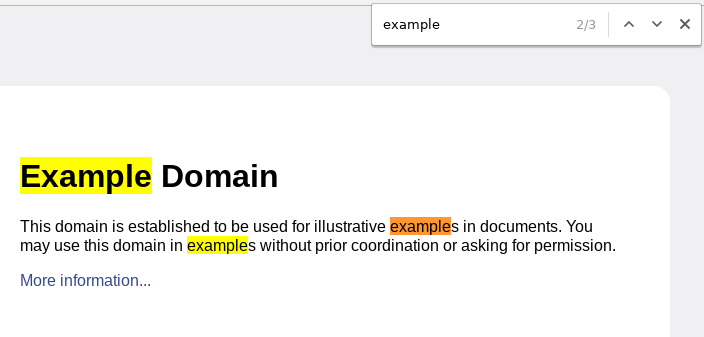
\includegraphics[width=0.6\textwidth]{../docs/browser-find-toolbar/chrome-find.png}
\caption{Google Chrome browser find tool}
\end{figure}

\begin{figure}[h]
\centering
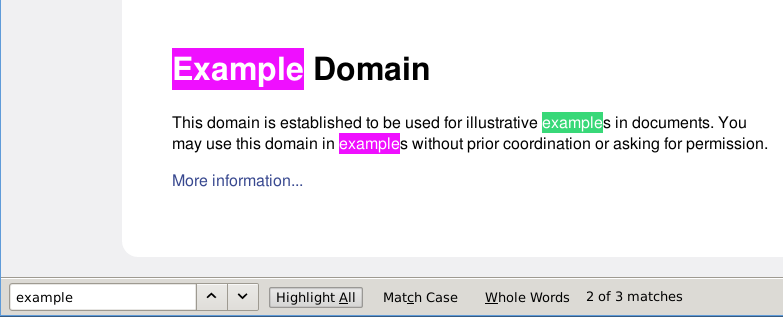
\includegraphics[width=0.6\textwidth]{../docs/browser-find-toolbar/firefox-find.png}
\caption{Mozilla Firefox browser find tool}
\end{figure}

There have been several attempts to implement this functionality via an extension. Most of them either don't work, are missing functionality (particularly support for regular expressions), are limited to certain websites, or are counter-intuitive and hard to use in general. 


%in which the project topic is described and set in the context of published literature, and the main results are briefly summarized (about five pages). 

%This chapter should include a clear and concise summary of your contributions (examples: adapting a suite of existing code; interpreting a theoretical algorithm; coding; testing; conducting an experiment) preferably as a bulleted list.

%The Introduction chapter should always provide a 'roadmap' to the report. Of course it should provide an introduction to the problem being considered, but it should also give some details of what you did - do not leave this to the conclusion. You should give forward references into the rest of the report - e.g., "In Chapter 2 how algorithms and heuristics are used to deal with approximate counting are discussed", "The design of the system is presented in Chapter 4", "In Chapter 3 the reasons for choosing to focus on the bounded-degree case of this problem are explained". 

%Your report will be read by markers throughout the School of Informatics. Do not assume that your marker is an expert in your subfield. Give some basics as well as the details. Also, make sure you point out what was involved in solving certain problems; this can help a non-expert judge the work involved. For instance: "The interpolation algorithm was implemented in C directly, rather than using the routines in Matlab". "In order to develop a user interface appropriate for the educational system, 4 prototypes were tested on 50 students". 

% Use passive voice: A and B were used. instead of I used A and B


\chapter{Background}
%  A brief introduction to browser extensions would be a good addition to an early part of the thesis. 
\chapter{Design}
\section{User Interface}


\chapter{Implementation}
% overall principles and aspects of particular interest, rather than minute details.

%You should always make it clear what was completed, and what was left as future work. If in doubt spell it out: tell us which bits of code you could find already written, which bits you had to do from scratch, which bits were routine, which bits were challenging (and why). 

\chapter{Evaluation}

\chapter{Conclusions}
% in which the main achievements are reviewed, and unsolved problems and directions for further work are presented.

% Bibliography section --- use \cite{P1} with BibTeX
\bibliographystyle{plain}
\bibliography{mybibfile}

\end{document}
